\chapter{Implementação}
\label{sec-implementacao}

Após a definição do escopo \ref{sec:escopo}, dos requisitos \ref{sec:requisitos-do-jogo}, do diagrama de classes \ref{sec:diagrama-de-classes}, da ideia do jogo \ref{sec:jogo}, do ferramental teórico e prático que será utilizado no desenvolvimento do trabalho \ref{sec-referencial} e uma motivação bem definida, temos uma base sólida para a implementação. Neste capítulo são apresentados os detalhes relacionados à arquitetura do programa e a implementação do software desenvolvido, bem como algumas das decisões de \textit{software} tomadas com base na seção anterior. O objetivo deste capítulo é fornecer uma visão clara e detalhada de como o software foi estruturado e construído, demonstrando as escolhas técnicas realizadas para atender aos requisitos definidos previamente. O código-fonte do jogo está disponível no Github \footnote{Super Labes World no Github \url{https://github.com/haskellman/Super-Labes-World}}.
% Além disso, serão discutidas as escolhas realizadas durante o desenvolvimento, evidenciando como essas funções se complementam.

Antes de começar um jogo em \textit{pixel art}, é importante definir o tamanho de cada \textit{tile}; os tamanhos mais comuns são (16 x 16), (32 x 32) e (64 x 64). Para esse trabalho, foi optado o tamanho (64 x 64) por ser possível adicionar mais detalhes em cada tile. É importante que todos os tiles presentes no jogo respeitem o mesmo tamanho para uma melhor harmonia visual e proporção de objetos.

\section{Arquitetura do Jogo}
\label{sec:arquitetura-do-jogo}
O desenvolvimento de um jogo envolve a integração de diversas camadas tecnológicas que, se não bem estruturadas, podem inviabilizar o software futuramente. Pensando em melhorar a estruturação do programa, foi projetada uma arquitetura em alto nível para melhor compreensão do código e seus componentes. A Figura \ref{fig:game-architecture} representa uma visão estática da implementação. O retângulo maior representa o jogo e dentro dele a sua lógica. A parte superior são os recursos que o jogo provê internamente, e a parte inferior corresponde aos recursos externos que são utilizados pelo jogo.

\begin{figure}[h!]
    \centering
    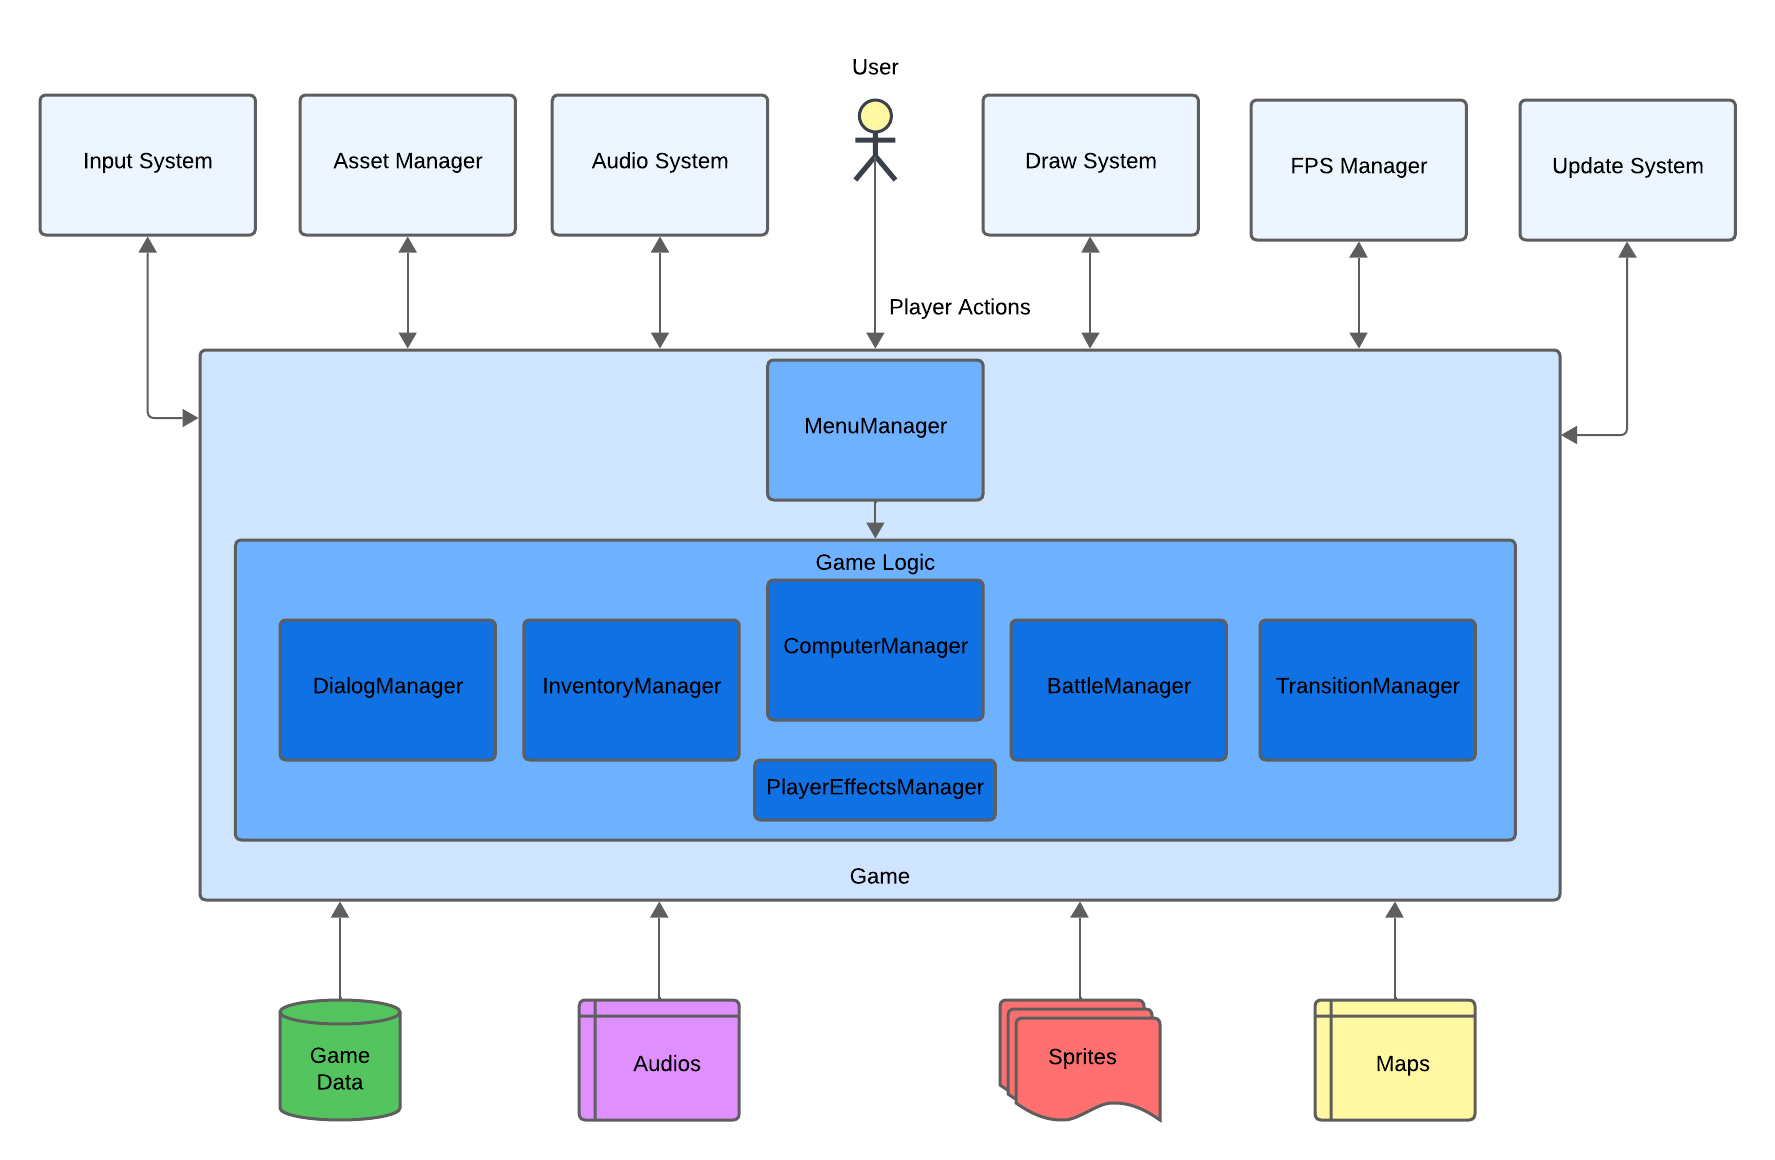
\includegraphics[width=1\linewidth]{figuras/game-architecture.png}
    \caption{Arquitetura do Super LabES World em alto nível}
    \label{fig:game-architecture}
\end{figure}

\clearpage
\section{Inicializando o Jogo}
\label{sec:principais-funcoes}
A primeira coisa a se fazer em um projeto Pygame é inicializá-lo invocando o método \textit{pygame.init()}. Isso inicializará todos os módulos do Pygame e permitirá chamadas de funções. Os \textit{sprites} mencionados na seção \ref{sec:aseprite} são uma peça fundamental na criação de jogos. No Pygame, \textit{sprites} podem ser representados pela classe nativa \textit{Sprite}; herdar essa classe base e adicionar os atributos e métodos que são do nosso interesse é muito útil. Outra classe importante para a criação de um jogo Pygame é a classe \textit{Group} que consiste de uma classe \textit{container} que possibilita adicionar objetos do tipo \textit{Sprite}. 

Utilizar essas classes em conjunto possibilita ao programador criar grupos de \textit{Sprites} que podem ser utilizados pelo programador para implementar comportamentos específicos. No Super Labes World, existem cinco tipos de grupos de \textit{sprites} que representam cinco comportamentos diferentes, podendo um \textit{sprite} pertencer a mais de um grupo simultaneamente. A listagem \ref{lst:game} apresenta a classe \textit{Game} onde são inicializados todos os grupos, variáveis e \textit{assets} do jogo.


\lstinputlisting[label=lst:game, caption=Classe \textit{Game}, language=Python, float=htpb]{codigos/game.py}

Os grupos no código acima têm os seguintes comportamentos:
\begin{itemize}
    \item \textit{\textbf{collision\_sprites: }}Grupo que contém todos os \textit{sprites} colidíveis do jogo;
    \item \textit{\textbf{character\_sprites: }}Grupo que contém todos os \textit{sprites} de personagens do game;
    \item \textit{\textbf{transition\_sprites: }}Grupo que contém todos os \textit{sprites} com comportamento de colisão;
    \item \textit{\textbf{dialogs\_sprites: }}Grupo que contém todos \textit{sprites} que geram uma caixa de diálogo ao colidir;
    \item \textit{\textbf{interaction\_sprites: }}Grupo que contém todos os \textit{sprites} do jogo que são interativos;
\end{itemize}

A classe \textit{Game} também é responsável por chamar as funções \textit{import\_assets} que carregarão todos os \textit{assets} do jogo para o programa, e a função \textit{setup}, que carrega o mapa para o jogo. Ao olharmos a arquitetura do jogo ilustrada na figura \ref{fig:game-architecture}, a classe \textit{Game} realiza a camada de \textit{Asset Manager} além de carregar os recursos da parte inferior da figura. 

\lstinputlisting[label=lst-import-assets, caption=Import Assets, language=Python, float=htpb]{codigos/import_assets.py}

O método \textit{import\_assets}, mencionado na listagem \ref{lst-import-assets} ,é encarregado de fazer a importação e alocação de todos os mapas e \textit{assets} do jogo. A atribuição desses \textit{assets} é feita através de um dicionário para melhor organização do código. Abaixo, na tabela \ref{tbl-especificacao-dicionario}, a especificação do dicionário é ilustrada, com as possíveis chaves e valores.

\begin{table}[h!]
	\caption{Tabela com a especificação dos dicionários de assets.}
	\label{tbl-especificacao-dicionario}
	\centering
	\renewcommand{\arraystretch}{2}
	\begin{small}
		\begin{tabular}{ | p{35mm} | p{35mm} | p{65mm} |}\hline \rowcolor{MidnightBlue}
                \hline
                Variável & Chave & Valor \\
                \hline
                \textit{tmx\_maps} & \textit{map\_name} & Arquivo TMX \\ 
                \hline
                \multirow{3}{4em}{overworld\_frames} 
                & \textit{characters} & \textit{Sprites} de personagems \\ 
                & \textit{water} & \textit{Sprites} de água \\ 
                & \textit{lake} & \textit{Sprites} das bordas do lago \\ 
                \hline
                \multirow{3}{4em}{fonts} 
                & \textit{dialog} & Fonte do diálogo \\ 
                & \textit{bold} & Fonte negrito \\ 
                & \textit{regular} & Fonte do inventário e computador \\ 
                & \textit{regular\_mid} & Fonte do inventário com tamanho 22 \\ 
                & \textit{regular\_big} & Fonte do inventário  com tamanho 34 \\ 
                \hline
                \multirow{3}{4em}{interface\_frames} 
                & \textit{interface} & \textit{Sprites} com os \textit{layouts} da interface \\ 
                & \textit{items} & \textit{Sprites} com os items do inventario \\ 
                & \textit{interactive\_objects} & \textit{Sprites} que tem algum tipo de animação ao interagir \\ 
                \hline

                \end{tabular}
	\end{small}
\end{table}

\clearpage
\lstinputlisting[label=lst-setup, caption=Setup, language=Python, float=htpb]{codigos/setup.py}

O método \textit{setup} tem a função de carregar para o jogo o mapa passado como parâmetro, além de inicializar os \textit{sprites} presentes nesse mapa. Essa função é chamada ao iniciar um novo jogo com o parâmetro do mapa inicial; também é chamada caso o jogador mude de mapa. Neste segundo caso, é necessário limpar os \textit{sprites} do mapa anterior. Logo após isso, a função executa uma série de \textit{loops} sobre todas as camadas do mapa criadas no editor de mapas, a fim de configurar todos os \textit{sprites} presentes no mapa em seus respectivos grupos. 
A listagem \ref{lst-setup} mostra como é feita essa associação para alguns \textit{sprites}. As demais atribuições são semelhantes a essa e podem ser vistas na tabela \ref{tbl-especificacao-sprites}.

\begin{table}[h!]
	\caption{Tabela especificando os tipos de \textit{sprites} presentes em Super Labes World}
	\label{tbl-especificacao-sprites}
	\centering
	\renewcommand{\arraystretch}{3}
	\begin{small}
		\begin{tabular}{ | p{37mm} | p{23mm}  | p{52mm} | p{30mm} | }\hline \rowcolor{MidnightBlue}
			\centering{\textbf{Classe}} & \centering{\textbf{Camadas}} & \textbf{Descrição} & \textbf{Grupos} \\\hline		
                \centering{\textit{Sprite}} & \centering{\textit{Terrain, Terrain Top, Terrain Objects}} & {Classe com os tiles da camada mais baixa sem colisões} & {\textit{all\_sprites}} \\\hline
                \centering{\textit{AnimatedSprite}} & \centering{\textit{Lake, Lake Edges}} & {Classe com tiles animados do lago sem colisão} & {\textit{all\_sprites}} \\\hline			
                \centering{\textit{CollidableSprite}} & \centering{\textit{Objects}} & {Classe com os sprites de objetos do jogo com colisão} & {\textit{all\_sprites, collision\_sprites}} \\\hline		
                \centering{\textit{InteractiveSprite}} & \centering{\textit{Interactive Objects}} & {Classe com os sprites com interação com colisão} & {\textit{all\_sprites, collision\_sprites, interactive\_sprites}} \\\hline	
                \centering{\textit{CollisionSprite}} & \centering{\textit{Collisions}} & {Classe com as colisões sem uma imagem} & {\textit{collision\_sprites}} \\\hline		
                \centering{\textit{CollidableDialogSprite}} & \centering{\textit{Dialogs}} & {Classe com os sprites de diálogo} & {\textit{dialog\_sprites}} \\\hline		
                \centering{\textit{TransitionSprite}} & \centering{\textit{Transitions}} & {Classe que armazena os sprites de transição sem imagem} & {\textit{transition\_sprites}} \\\hline		
                \centering{\textit{Player}} & \centering{\textit{Entities}} & {Classe do jogador principal} & {\textit{all\_sprites}} \\\hline	
                \centering{\textit{Character}} & \centering{\textit{Entities}} & {Classe para representar as entidades de personagens do jogo} & {\textit{all\_sprites, collision\_sprites, characters\_sprites}} \\\hline	
		\end{tabular}
	\end{small}
\end{table}
% \begin{table}[h!]
% 	\caption{Tabela especificando os tipos de \textit{sprites} presentes em Super Labes World}
% 	\label{tbl-especificacao-sprites}
% 	\centering
% 	\renewcommand{\arraystretch}{3}
% 	\begin{small}
% 		\begin{tabular}{ | p{37mm} | p{23mm}  | p{52mm} | p{30mm} | }\hline \rowcolor{MidnightBlue}
% 			\centering{\textbf{Classe}} & \centering{\textbf{Camadas}} & \textbf{Descrição} & \textbf{Grupos} \\\hline	
%                 \centering{\textit{Character}} & \centering{\textit{Entities}} & {Classe para representar as entidades de personagens do jogo} & {\textit{all\_sprites, collision\_sprites, characters\_sprites}} \\\hline	
% 		\end{tabular}
% 	\end{small}
% \end{table}

\clearpage
\section{Game Loop do Super Labes World}
\label{sec:game-loop-super-labes-world}
% game loop

Como discutimos na seção \ref{sec:game-loop}, o \textit{game loop} é o núcleo do jogo e é responsável por manter o jogo em execução contínua até que o jogador feche o programa ou o jogo termine. Nele, são continuamente processadas tarefas predefinidas no código do jogo. O \textit{game loop} é o responsável integralmente pela camada de lógica do programa da arquitetura da figura \ref{fig:game-architecture}.

\lstinputlisting[label=lst-game-loop, caption=Main, language=Python, float=htpb]{codigos/game_loop.py}

A função ilustrada na listagem \ref{lst-game-loop} implementa o \textit{Game Loop} do Super LabES World, composto pelos seguintes passos:
\begin{enumerate}
    \item Preencher a área do mapa que não contém tiles com preto (linha 6);
    \item Atualizar o valor do \textit{delta time} (linha 7), relacionado ao \textit{fps manager} da arquitetura do jogo. Sua importância foi explicada na seção \ref{sec:delta-time};
    \item Verificar o evento de fechar o jogo (linhas 8 a 11);
    \item Chamar a função de \textit{input}, que lida com a entrada de controles do jogador (linha 14);
    \item Verificar se o jogador colidiu com um \textit{sprite} de transição (linha 15). Se for o caso então é chamada a função \textit{setup} com os devidos parâmetros do mapa a ser transicionado;
    \item Verificar se o jogador colidiu com alguma caixa de diálogo (linha 16). Se sim então é chamado a função para criar o diálogo com a mensagem;
    \item Atualizar todos os \textit{sprites} da tela (linha 17), relacionado ao \textit{update system} da arquitetura do jogo. Essa linha chama o método \textit{update} de todos os \textit{sprites} contidos no \textit{Group all\_sprites}; 
    \item Desenhar todos os \textit{sprites} da tela (linha 20), relacionado ao \textit{draw system} da arquitetura;
    \item Verificar se tem algum \textit{overlay} (sobreposição) na tela do jogo, as variáveis que tratam isso foram criadas na listagem \ref{lst:game} e são usadas aqui no \textit{loop} principal. Para cada uma dessas variáveis existe a instanciação de sua classe de sobreposição, sendo cinco as possíveis telas de sobreposições no jogo:
        \begin{itemize}
        \item \textit{\textbf{dialog\_open: }} Verdadeiro quando o jogador aperta \textit{spacebar} próximo a uma personagem do jogo. Nesse caso sai do \textit{loop} principal e vai para o \textit{loop} da classe \textit{Dialog};
        \item \textit{\textbf{inventory\_open: }}Verdadeiro caso o jogador aperte a tecla ''i'', troca o contexto do \textit{loop} principal para o \textit{loop} da classe \textit{Inventory}; 
        \item \textit{\textbf{computer\_open: }} Verdadeiro quando o jogador aperta \textit{spacebar} próximo a \textit{InteractiveObject} com o \textit{item\_id} = \textit{computer}. Então troca de contexto do \textit{loop} principal para o \textit{loop} da classe \textit{Computer};
        \item \textit{\textbf{battle\_open: }}  Verdadeiro quando o jogador responde sim para um desafio de um personagem. Nesse caso troca-se de contexto para a classe \textit{Battle};
        \item \textit{\textbf{choose\_dialog\_open: }} Verdadeiro ao fim de um diálogo de um personagem que contém questões e que não foi derrotado. Troca o contexto para a classe \textit{Choose\_dialog};
    \end{itemize}
\end{enumerate}


% input
\section{Entrada de Controles}
A entrada de controles \textit{(input system)}, da arquitetura do Super Labes World é feita sempre através de um método chamado \textit{input}. As classes que possuem esse método implementado em seu escopo, além da classe principal, são as classes \textit{Player}, que lida com a movimentação do personagem, e as classes de sobreposição, citadas na seção anterior, que lidam com os controles do jogador em sua respectiva tela. Nessa seção serão detalhadas as três possíveis formas de como é feito no Super Labes World.

O método \textit{input} da listagem \ref{lst-overlay-input} é relativo à classe principal do jogo, ele lida com os comandos de inventário e interação do jogador. A princípio, verifica se o jogador não está em estado bloqueado, ou seja, em um diálogo, ou em alguma janela de sobreposição. Após isso, a função encarrega-se de lidar com os possíveis comandos, sendo eles:
\begin{itemize}
    \item \textbf{Tecla I: }Abre o inventário e coloca o player no estado bloqueado;
    \item \textbf{Tecla ESC: }Fecha as interfaces de inventário, computador e tira o jogador do estado bloqueado;
    \item \textbf{Tecla \textit{Spacebar}: }A tecla de interação do jogador, quando pressionada é verificado se o jogador está perto a um personagem, ou a um objeto interativo. Quando for o caso a função leva para o respectivo tratamento.
\end{itemize}

\lstinputlisting[label=lst-input, caption=Input, language=Python, float=htpb]{codigos/input.py} 

Outra importante função input é relativa à  movimentação do \textit{player}. Após a chamada do método \textit{all\_sprites.update()} na linha 17 da listagem \ref{lst-game-loop}, o programa chama o método \textit{update} de todas as classes contidas neste grupo, incluindo a classe \textit{Player}. A listagem \ref{lst-player-animation} mostra as funções responsáveis pela movimentação do jogador.

\lstinputlisting[label=lst-player-animation, caption=Player movement, language=Python, float=htpb]{codigos/player_animation.py}
\begin{itemize}
    \item \textit{\textbf{update:}} Função que chama todos os métodos necessários para a movimentação do personagem principal;
    \item \textit{\textbf{animate:}} Função que intercala os frames de forma a criar uma impressão de animação como explicado na seção \ref{sec:aseprite};
    \item \textit{\textbf{input:}} Função que retorna um vetor cartesiano [x, y] normalizado, referente a direção das teclas que o jogador pressionou;
    \item \textit{\textbf{move:}} Realiza a movimentação do personagem de acordo com o vetor obtido anteriormente e uma velocidade predefinida.
\end{itemize}

Por fim, o método \textit{input} da classe \textit{Inventory},  que é uma das possíveis sobreposições do jogo. Esse \textit{input} está em vigor quando o \textit{game loop} troca de contexto para a classe \textit{Inventory} (quando o jogador pressiona '' I ''). Diferentemente das outras funções \textit{input}, aqui existe um limite para as opções a serem escolhidas pelo jogador, na figura \ref{fig:inventory} é possível visualizar o inventário, representado como uma matriz 10 x 3, ou seja, 30 posições possíveis. É feito uso do operador \% (resto da divisão inteira) para limitar o valor de índice ao tamanho do inventário. Essa lógica de índice também é aplicada a outras telas, como \textit{Battle}, \textit{Computer}, \textit{Choose\_dialog}. A listagem a seguir \ref{lst-overlay-input} mostra o método \textit{input} da classe \textit{Inventory}. 

\lstinputlisting[label=lst-overlay-input, caption=\textit{Input} da classe \textit{Home}, language=Python, float=htpb]{codigos/overlay_input.py}



\clearpage
\section{Sistema de Batalhas}
O jogador pode entrar em uma batalha através da resposta 'sim' a um desafio proposto por um professor, veja a interface de escolha na figura \ref{fig:choose-dialog}, e a ilustração da batalha na figura \ref{fig:battle}. O programa bloqueia a entrada de comandos do \textit{game loop} principal e muda para o contexto da classe \textit{Battle}. O loop do contexto de \textit{Battle} é ilustrado a seguir na listagem \ref{lst-update-battle}.

\lstinputlisting[label=lst-update-battle, caption=Loop da classe \textit{Battle}, language=Python, float=htpb]{codigos/update_battle.py}

As funções desse \textit{loop} realizam as seguintes ações:
\begin{enumerate}
    \item \textit{\textbf{battle\_timer.update:}} Atualiza a contagem de tempo na batalha;
    \item \textbf{\textit{check\_end\_battle:}} Verifica se o fim da batalha chegou, ou seja, todas as questões foram respondidas, ou o jogador errou 30\% do total de perguntas. Chama a função de \textit{callback} para o \textit{loop} principal com o resultado obtido;
    \item \textbf{\textit{input: }} Captura a entrada de comandos do jogador e lida com os índices, similar ao menu inventário explicado em \ref{lst-overlay-input};
    \item \textbf{\textit{display\_surface.blit:}} Desenha o background da batalha na tela;
    \item \textbf{\textit{draw\_rectangles:}} Função que desenha os retângulos de opções de resposta do jogador;
    \item \textbf{\textit{draw\_questions:}} Função que desenha na tela o texto da pergunta atual;
    \item \textbf{\textit{draw\_answers:}} Função que desenha o texto da resposta de acordo com a opção que o jogador está;
    \item \textbf{\textit{draw\_character\_info:}} Função que desenha as informações do professor na tela (nome e level);
    \item \textbf{\textit{draw\_characters:}} Função que realiza o desenho e a animação dos dos personagens nessa tela será mais detalhada a seguir;
    \item \textbf{\textit{draw\_dialog:}} Função que desenha o diálogo do professor ao responder a questão.
\end{enumerate}
\clearpage

Na batalha, o jogador pode selecionar uma entre quatro opções de resposta para cada pergunta. Para que o jogador tenha um \textit{feedback} visual da alternativa selecionada, é utilizado o método \textit{blit}. Esse método do Pygame permite combinar imagens na tela ao usar o parâmetro opcional \textit{special\_flags}. A figura \ref{fig:blit-example} mostra o resultado obtido da função apresentada na listagem \ref{lst-draw-rectangles}.

\begin{figure}[h!]
    \centering
    
\includegraphics[width=1\linewidth]{figuras/blit_example.png}
    \caption{Exemplo do funcionamento do método \textit{blit}}
    \label{fig:blit-example}
\end{figure}

\lstinputlisting[label=lst-draw-rectangles, caption=Desenho dos retângulos de resposta da classe \textit{Battle}, language=Python, float=htpb]{codigos/draw_rectangles.py}

A função \textit{check\_answer} (listagem \ref{lst-check-answer}) verifica a resposta do jogador. Ela é chamada quando o jogador responde a uma pergunta, ou seja, pressiona a tecla \textit{Enter} em uma das opções. A função atribui \textit{True} ou \textit{False} à variável \textit{error\_mode}, indicando se a resposta está correta ou errada, respectivamente. Além disso, emite um som e escolhe um texto diferente para respostas certas e erradas, para emitir um rápido \textit{feedback} ao jogador.

\lstinputlisting[label=lst-check-answer, caption=Função chamada ao jogador escolher uma opção na batalha, language=Python, float=htpb]{codigos/check_answer.py}


\clearpage
\section{Personagens}
\label{sec:personagens}
Os personagens de um jogo são uma peça fundamental, especialmente para um jogo do gênero RPG. Eles desempenham um papel central na construção da experiência narrativa e interativa e enriquecem fortemente a ambientação do jogo. Esse capítulo vai abordar em mais detalhes como foi feita a criação de personagens no Super LabES World.

Os \textit{sprites} dos personagens do jogo foram desenhados na ferramenta Aseprite, discutida na seção \ref{sec:aseprite} e exportados para o formato PNG (Portable Network Graphics). Cada \textit{sprite} de personagem tem o tamanho 512 x 512, mas no programa essa imagem é subdividida em 16 quadrados de tamanhos iguais 128 x 128, como mostra a figura \ref{fig:player-animation}.

A adição de personagens ao jogo é feita pela ferramenta Tiled, apresentada na seção \ref{sec:tiled}. No Tiled existe um recurso chamado \textit{Insert Point}, os pontos são os objetos mais simples possíveis de serem adicionados a um mapa. Esses pontos representam apenas uma localização e não podem ser redimensionados ou girados, mas é possível atribuí-los com metadados. Esses metadados podem ser utilizados no Pygame para a identificação de cada personagem. Em nosso caso, os metadados inseridos foram os seguintes:
\begin{itemize}
    \item \textbf{\textit{character\_id: }} Identificador do personagem. Todas as características do personagem (diálogos, \textit{frames}, questões, etc) são dependentes desse \textit{id};
    \item \textbf{\textit{direction: }}Define qual é a direção inicial do jogador;
    \item \textbf{\textit{pos:}} Contém o mapa anterior que o \textit{player} estava antes da transição. Isso é necessário porque todo mapa contém pelo menos duas possíveis transições (ida e volta). Essa variável então é usada para diferenciar cada posição do jogador e o programa conseguir desenhar o jogador na posição correta. (Propriedade é relativa somente ao player);
\end{itemize}

Essas propriedades podem ser vistas na figura \ref{fig:tiled-player-properties}, na figura \ref{fig:tiled-house} é possível ver como os personagens foram inseridos no jogo.
\begin{figure}[h!]
    \centering
    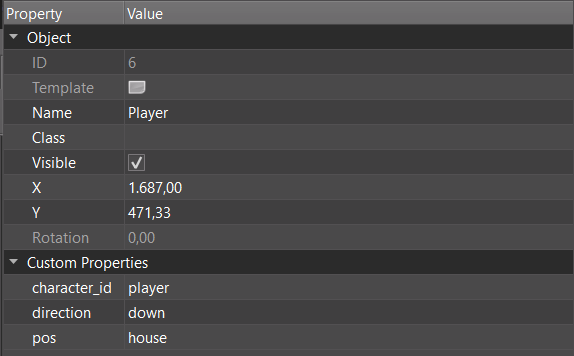
\includegraphics[width=0.5\linewidth]{figuras/tiled-player-properties.png}
    \caption{Propriedades da Entidade Player no Tiled}
    \label{fig:tiled-player-properties}
\end{figure}


\begin{landscape}
    \begin{figure}[h!]
        \centering
        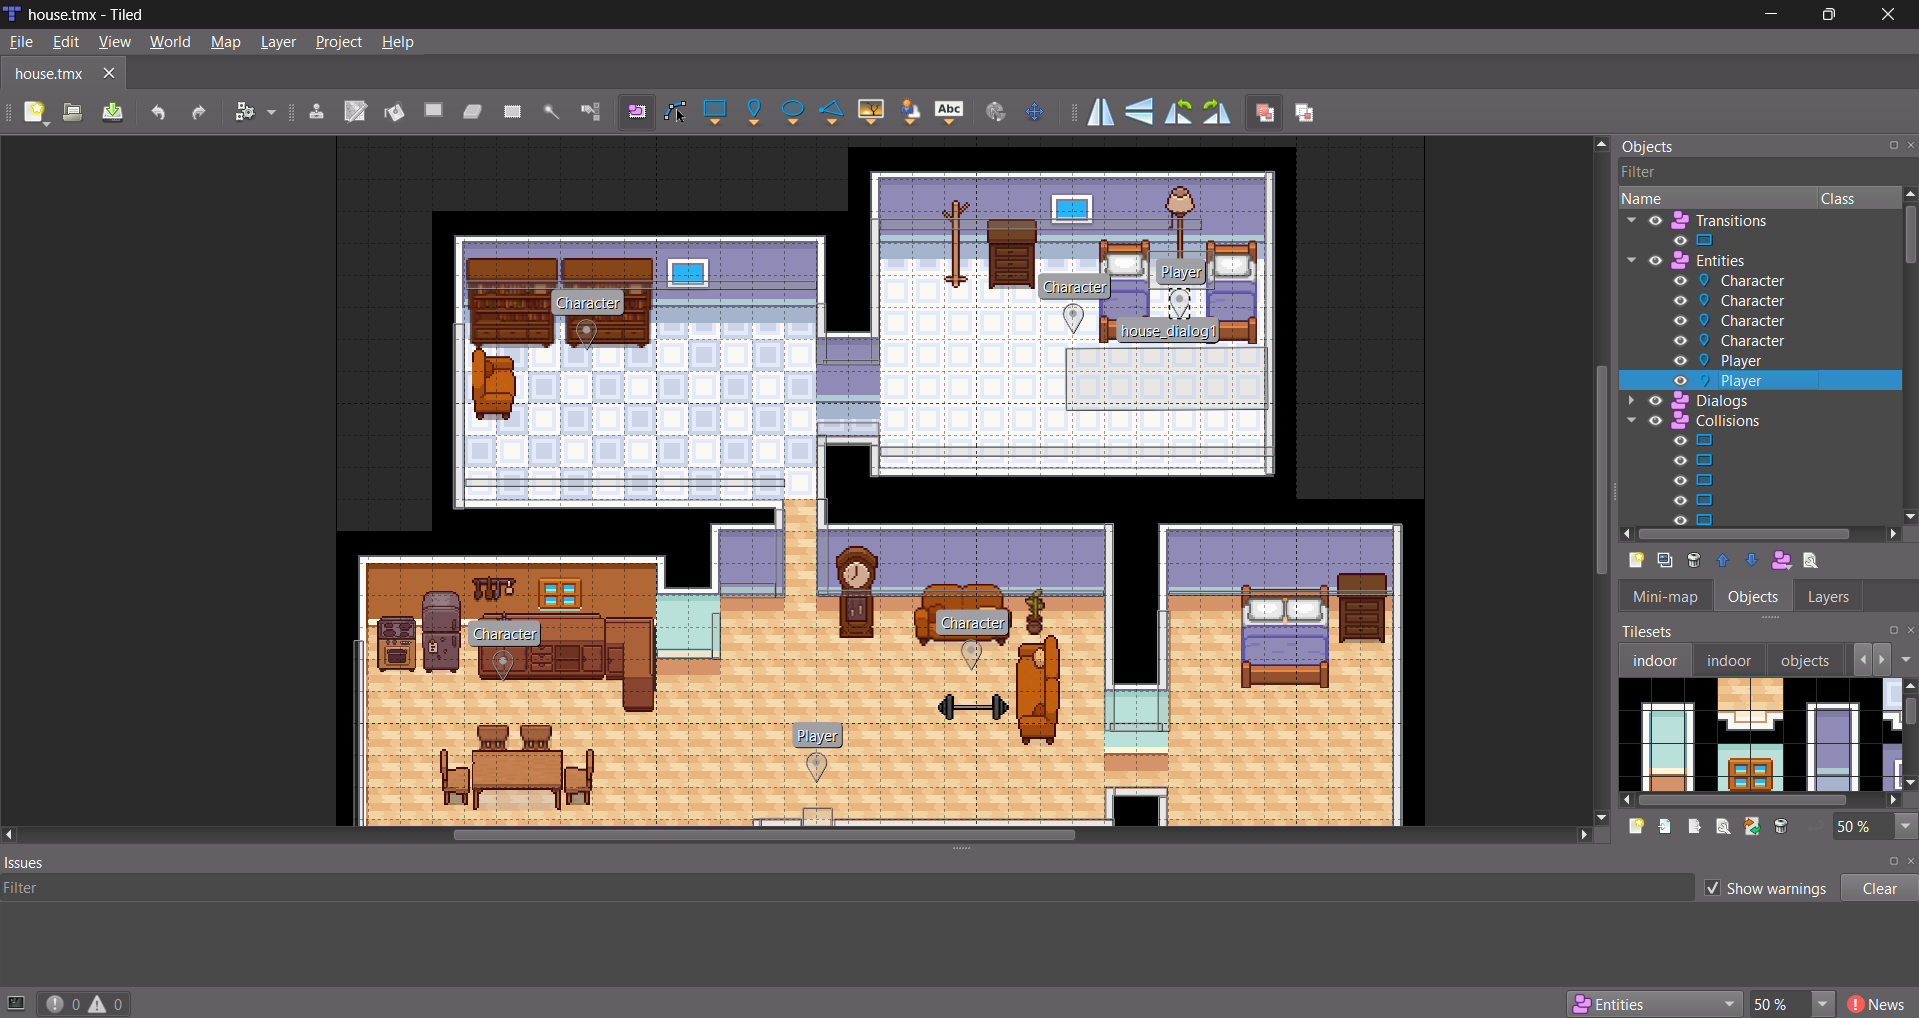
\includegraphics[width=1\linewidth]{figuras/tiled-house.png}
        \caption{Posicionamento de Objetos no Software Tiled }
        \label{fig:tiled-house}
    \end{figure}
\end{landscape}


\clearpage
Animação, como explicado na seção \ref{sec:aseprite}, é uma ilusão gerada pela sequência de imagens alternadas a uma determinada velocidade. No Super Labes World, para aplicar essa técnica, é criado um dicionário, cuja chave é o nome do estado em que o jogador se encontra e o valor, um vetor de imagens relacionadas aos possíveis estados. A figura ilustra como a associação da imagem é feita no código:
\begin{figure}[h!]
    \centering
    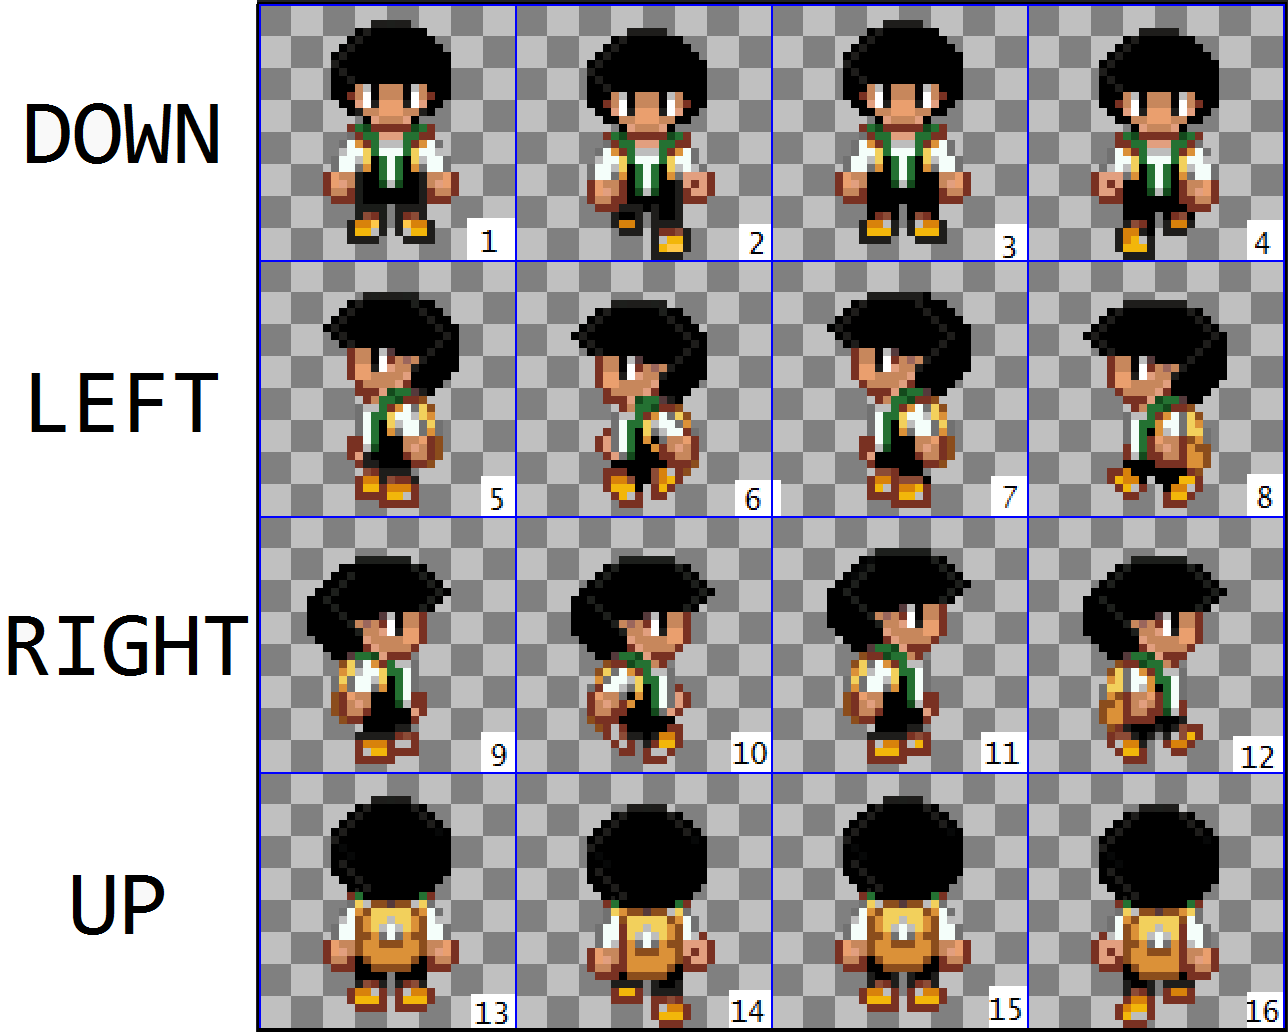
\includegraphics[width=1\linewidth]{figuras/player-animation.png}
    \caption{\textit{Sprite} de Animação dos \textit{Player} }
    \label{fig:player-animation}
\end{figure}

Cada chave do dicionário contém quatro imagens (frames). Também são criados quatro estados adicionais com o sufixo \textit{''idle''} (parado) correspondentes a cada direção. Isso é feito para que, quando o jogador interrompa a movimentação, o programa mude o \textit{frame} para a direção atual do jogador, mas na posição parado. 
\begin{enumerate}
    \item \textit{\textbf{down:}} Mantém as imagens 1, 2, 3 e 4;
    \item \textit{\textbf{down\_idle:}} Mantém a imagem 1;
    \item \textit{\textbf{left:}} Mantém as imagens 5, 6, 7 e 8;
    \item \textit{\textbf{left\_idle:}} Mantém a imagem 5;
    \item \textit{\textbf{right:} Mantém as imagens 9, 10, 11 e 12};
    \item \textit{\textbf{right\_idle:}} Mantém a imagem 9;
    \item \textit{\textbf{up:}} Mantém as imagens 13, 14, 15 e 16 ;
    \item \textit{\textbf{up\_idle:}} Mantém a imagem 13;
\end{enumerate}

% % detalhar mais aqui
% Para realizar a movimentação do personagem principal no código, foram criados os seguintes métodos:
% \lstinputlisting[label=lst-player-animation, caption=Player movement, language=Python, float=htpb]{codigos/player_animation.py}
% \begin{itemize}
%     \item \textit{\textbf{input:}}  Retorna um vetor [x, y] direcional normalizado relativo as teclas que o jogador jogador pressionou;
%     \item \textit{\textbf{move:}} Realiza a movimentação do personagem de acordo com o vetor obtido anteriormente;
%     \item \textit{\textbf{update:}} Função que é chamada no \textit{loop} principal do jogo, é a partir dela que todas as anteriores são chamadas;

% \end{itemize}

\clearpage

\section{Extensibilidade}
Jogos do gênero RPG podem ser bastante extensos, oferecendo centenas de horas de jogo. Alguns recebem constantes atualizações com melhorias e novos conteúdos. Por esse motivo, esta seção será dedicada a programadores interessados em expandir o Super LabES World.

\subsection{Novos Personagens}
Para expandir o jogo, é essencial dispor de novos \textit{sprites} de personagens. Existem diversos softwares especializados em Pixel Art que facilitam o processo de criação. Todos os \textit{sprites} de personagens do Super Labes World foram desenhados em uma área quadrada de 128 x 128 pixels. Recomenda-se seguir esse padrão para manter a coesão estética.

Para incluir esses \textit{sprites} ao jogo, basta colocá-los na pasta \textit{characters} do projeto. Todos os \textit{sprites} dessa pasta são carregados automaticamente pelo programa. Após isso, usando o editor de mapas Tiled, será definido o local onde o personagem será posicionado, conforme explicado na seção \ref{sec:personagens}. Para adicionar as informações do personagem ao jogo, deve-se incluir ao dicionário \textit{CHARACTERS\_DATA}, presente no arquivo \textit{game\_data}, com as informações no formato apresentado a seguir, na listagem \ref{lst-add-character}:

\lstinputlisting[label=lst-add-character, caption=Formato de dados para inclusão de personagems no jogo, language=Python, float=htpb]{codigos/add_character.py}

\clearpage
\subsection{Novas Batalhas}
Para adicionar novas batalhas aos personagens, basta inserir, no campo ``questions'' da listagem \ref{lst-add-character}, qualquer quantidade de perguntas, seguindo o padrão apresentado na listagem \ref{lst-add-question}.

\lstinputlisting[label=lst-add-question, caption=Formato de dados para inclusão de batalhas no jogo, language=Python, float=htpb]{codigos/add_question.py}

O campo ``\textit{link}'' da listagem \ref{lst-add-question} indica qual material de apoio disponível na web a questão está relacionada. Esse campo é preenchido a partir de um dicionário de links, no seguinte da listagem \ref{lst-add-link}.

\lstinputlisting[label=lst-add-link, caption=Formato de dados para inclusão de \textit{links} ao jogo, language=Python, float=htpb]{codigos/add_link.py}

\clearpage
\subsection{Novos Mapas} 
Os mapas foram criados usando o \textit{software} Tiled, como já mencionado anteriormente. Para interligar esses mapas no jogo, foi criada uma camada de objetos para posicionar as transições. As transições no programa são definidas como retângulos com metadados de origem e destino. A figura \ref{fig:map-transiction} ilustra como a transição foi posicionada, e a figura \ref{fig:transiction-properties} mostra as propriedades da transição para a sala do chefe Vitor, como exemplo.

\begin{figure}[h!]
    \centering
    \begin{minipage}{0.45\textwidth}
        \centering
        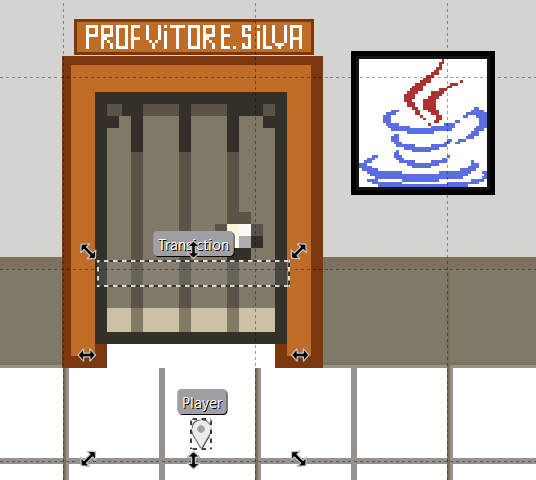
\includegraphics[width=\textwidth]{figuras/map-transiction.png} % Substitua pelo caminho da imagem
        \caption{Adicionando transição ao mapa Tiled}
        \label{fig:map-transiction}
    \end{minipage}\hfill
    \begin{minipage}{0.45\textwidth}
        \centering
        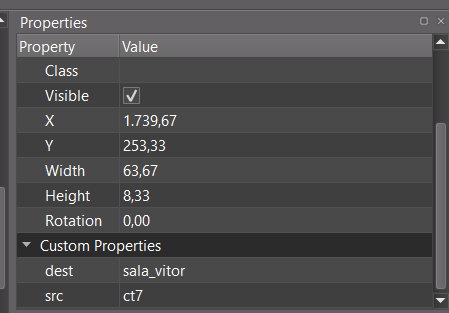
\includegraphics[width=\textwidth]{figuras/transition-properties.png} % Substitua pelo caminho da imagem
        \caption{Figura ilustrando a inclusão dos metadados \textit{dest} e \textit{src} para o retângulo}
        \label{fig:transiction-properties}
    \end{minipage}
    \caption{Incluindo mapas ao jogo}
    \label{fig:side_by_side}
\end{figure}

\clearpage
\section{Conclusões do Capítulo}
Neste capítulo, entramos em detalhes sobre a implementação do Super Labes World. Primeiramente, foi ilustrada a arquitetura geral do jogo com o objetivo de facilitar a compreensão do sistema como um todo. Após, foi detalhada a implementação das principais funções que estruturam o jogo, sendo divididas em i) carregamento do jogo, ii) \textit{game loop}, iii) controles do jogo, iv) batalhas, v) personagens e, por fim, vi) extensibilidade, onde abordamos como os desenvolvedores podem expandir o jogo.

%acho que poderíamos ter uma seção de fechamento deste capítulo. O que foi feito e o que leitor pode esperar para  o próximo